\documentclass[11pt, a4paper]{article}

% --- 1. Formatting as per guidelines ---
% Set 1-inch margins
\usepackage[a4paper, margin=1in]{geometry}
\usepackage{setspace}
% \setstretch{1.5}
% Set 11pt font (done in documentclass)

% --- 3. Math & Theorem Packages ---
\usepackage{amsmath}
\usepackage{amssymb}
\usepackage{amsthm}
\usepackage{tikz}
\usetikzlibrary{positioning, arrows.meta}
\usepackage{float}
\usepackage{datetime2}
\usepackage{fancyhdr}
\usepackage{booktabs}
\usepackage{indentfirst}

% Define theorem-like environments
\theoremstyle{definition}
\newtheorem{definition}{Definition}[section]
\theoremstyle{plain}
\newtheorem{theorem}{Theorem}[section]
\newtheorem{lemma}[theorem]{Lemma}
\newtheorem{corollary}[theorem]{Corollary}
\newtheorem{conjecture}[theorem]{Conjecture}

% --- 4. Other Packages ---
\usepackage{xcolor} % Required for coloring text
% Custom command to print citations in red, as per user request
\newcommand{\redcite}[1]{\textcolor{red}{[#1]}} 

% Custom command for theorem/important results citation: [Number, Author Name]
\newcommand{\theoremcite}[2]{\textcolor{red}{[#1]}, #2} 

\usepackage{hyperref} % For links, must be loaded late
\hypersetup{
    colorlinks=true,
    linkcolor=black,
    citecolor=black,
    urlcolor=blue,
    pdftitle={The Theory of Graph Minors},
    pdfauthor={Manish Acharya},
}

% --- 5. Page Numbering ---
\pagestyle{plain} 
\pagenumbering{arabic}

\newcommand{\lastupdated}{Last updated: \DTMtoday}

\title{\LARGE\bfseries The Theory of Graph Minors}
\author{\Large Manish Acharya}
\date{}

\begin{document}

% --- Title Block ---

\maketitle

\thispagestyle{plain}
\renewcommand{\footrulewidth}{0pt}

\begingroup
\renewcommand{\thefootnote}{}
\footnotetext{\lastupdated}
\addtocounter{footnote}{-1}
\endgroup


\vspace{1.5em}

% --- Introduction ---
\section*{Introduction}
\label{sec:introduction}

The study of graph theory is fundamentally concerned with the structural properties of graphs. A powerful and abstract way to analyze this structure is to understand how graphs relate to simpler, more fundamental graphs. The theory of graph minors provides such a framework, defining a relationship that is arguably more profound than the subgraph relationship. At its core, a graph $H$ is a minor of a graph $G$ if $H$ can be derived from $G$ through a sequence of two fundamental operations: edge deletion, and edge contraction. 

This minor relation, defines a partial order on the set of all finite graphs. This perspective allows us to classify entire infinite families of graphs. For instance, the set of all planar graphs is a family that is \textbf{closed} under this minor operation; it is impossible to perform these operations on a planar graph and create a non-planar one. Such families are called \textbf{minor-closed} families.

A primary theme in the field, and the central focus of this paper, is the characterization of these infinite, minor-closed families by a finite set of \textbf{forbidden minors}. The foundational example is \textbf{Wagner's Theorem}, which re-contextualized Kuratowski's 
earlier planarity characterization: a graph is planar if and only if it does not contain 
$K_5$ or $K_{3,3}$ as a minor \redcite{9}. This single result demonstrates the power of 
the minor concept. The entire infinite class of planar graphs can be completely defined by 
just two forbidden structures.

The remainder of this paper is organized as follows. Section~1 introduces the minor operations
and the definition of minor-closed families, along with illustrative examples. Section~2 traces the
historical development from Kuratowski’s subdivision characterization of planarity to Wagner’s
forbidden-minor formulation and the emergence of \textbf{Hadwiger’s Conjecture}. Section~3 examines
Wagner’s Theorem and the structural ideas behind its proof. Section~4 presents the
\textbf{Robertson--Seymour Graph Minor Theorem} and explains the well-quasi-ordering framework
and its finite forbidden-minor corollary. Section~5 highlights some applications. A short conclusion closes the paper.

% --- Definitions ---
\section{Fundamental Definitions}
\label{sec:definitions}

To formalize the study of graph minors, we assume familiarity with the basic graph operations of vertex deletion ($G-v$) and edge deletion ($G-e$). These two operations, alone or in sequence, define the \textbf{subgraph} relationship: every subgraph is obtained only by these deletions. The addition of a third operation, edge contraction, is what distinguishes the minor relation and gives it its unique power.

\begin{definition}[Edge Contraction]
\label{def:contraction}
For a graph $G$ and an edge $e = \{u, v\} \in E(G)$, the contraction of $e$, denoted $G \cdot e$ (or $G/e$), results in a new graph $G'$. The two vertices $u$ and $v$ are merged into a single new vertex $w$. This new vertex $w$ is adjacent to every vertex $z$ that was a neighbor of either $u$ or $v$ in $G$ (excluding $u$ and $v$ themselves). The resulting graph is simplified by suppressing any loops or parallel edges that may be created.
\end{definition}

Since any sequence of vertex and edge deletions yields a subgraph, and the minor operation includes all deletions, it follows that every subgraph is a minor of the original graph. However, since the subgraph relationship does not permit edge contraction, not every minor is a subgraph. This makes the minor relation a more general and structurally powerful way to relate graphs. With these operations, we can formally define a graph minor.

\begin{definition}[Graph Minor]
A graph $H$ is a \textbf{minor} of a graph $G$ (written $H \preceq G$) if a copy of $H$ can be obtained from $G$ by deleting and/or contracting edges of $G$.
\end{definition}

% An alternative and often useful way to think about a minor $H$ within $G$ is as a collection of disjoint, connected subgraphs of $G$. Each vertex $v \in V(H)$ corresponds to a connected subgraph $G_v \subseteq G$, such that all these $G_v$ subgraphs are pairwise vertex-disjoint. For every edge $\{u, v\} \in E(H)$, there must be an edge in $G$ between a vertex in $G_u$ and a vertex in $G_v$. The graph $H$ is then formed by contracting each $G_v$ into a single vertex.

% --- Figure ---
\begin{figure}[H]
\centering
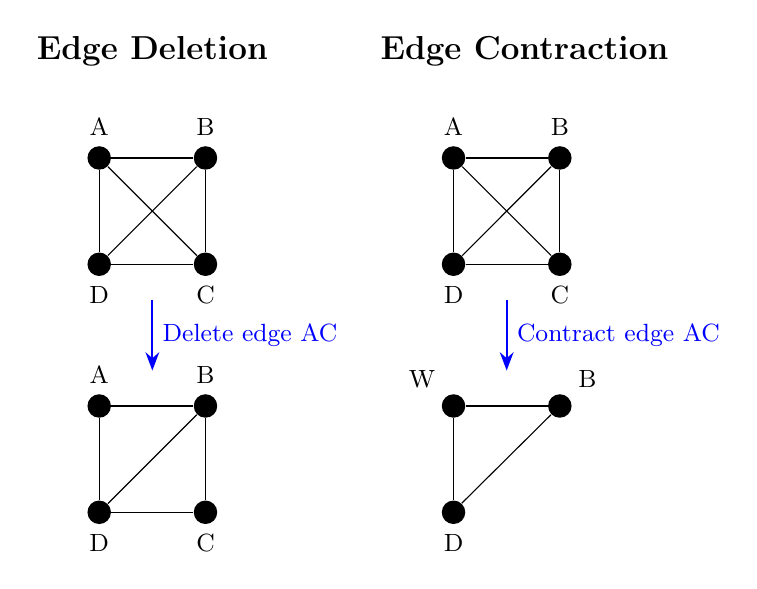
\begin{tikzpicture}[
    vertex/.style={circle,fill=black,inner sep=3pt},
    every node/.style={font=\small},
    scale=0.9
]
% Left side - Edge Deletion
\node[font=\large\bfseries] at (0.75,3.5) {Edge Deletion};
% Top graph
\begin{scope}
    \node[vertex,label={above:A}] (A1) at (0,2) {};
    \node[vertex,label={above:B}] (B1) at (1.5,2) {};
    \node[vertex,label={below:D}] (D1) at (0,0.5) {};
    \node[vertex,label={below:C}] (C1) at (1.5,0.5) {};
    
    \draw (A1) -- (B1);
    \draw (A1) -- (D1);
    \draw (B1) -- (C1);
    \draw (D1) -- (C1);
    \draw (A1) -- (C1);
    \draw (D1) -- (B1);
\end{scope}
% Arrow with text
\draw[-Stealth, thick, blue] (0.75,0) -- (0.75,-1) 
    node[midway,right,align=left,font=\small] {Delete edge AC};
% Bottom graph after deletion
\begin{scope}[yshift=-3.5cm]
    \node[vertex,label={above:A}] (A2) at (0,2) {};
    \node[vertex,label={above:B}] (B2) at (1.5,2) {};
    \node[vertex,label={below:D}] (D2) at (0,0.5) {};
    \node[vertex,label={below:C}] (C2) at (1.5,0.5) {};
    
    \draw (A2) -- (B2);
    \draw (A2) -- (D2);
    \draw (B2) -- (C2);
    \draw (D2) -- (C2);
    % AC edge deleted
    \draw (D2) -- (B2);
\end{scope}
% Right side - Edge Contraction
\node[font=\large\bfseries] at (6,3.5) {Edge Contraction};
% Top graph
\begin{scope}[xshift=5cm]
    \node[vertex,label={above:A}] (A3) at (0,2) {};
    \node[vertex,label={above:B}] (B3) at (1.5,2) {};
    \node[vertex,label={below:D}] (D3) at (0,0.5) {};
    \node[vertex,label={below:C}] (C3) at (1.5,0.5) {};
    
    \draw (A3) -- (B3);
    \draw (A3) -- (D3);
    \draw (B3) -- (C3);
    \draw (D3) -- (C3);
    \draw (A3) -- (C3);
    \draw (D3) -- (B3);
\end{scope}
% Arrow with text
\draw[-Stealth, thick, blue] (5.75,0) -- (5.75,-1) 
    node[midway,right,align=left,font=\small] {Contract edge AC};
% Bottom graph after contraction
\begin{scope}[xshift=5cm,yshift=-3.5cm]
    \node[vertex,label={above left:W}] (AC) at (0,2) {};
    \node[vertex,label={above right:B}] (B4) at (1.5,2) {};
    \node[vertex,label={below:D}] (D4) at (0,0.5) {};
    
    \draw (AC) -- (B4);
    \draw (AC) -- (D4);
    \draw (B4) -- (D4);
\end{scope}
\end{tikzpicture}
\caption{Graph minor operations}
\label{fig:graph-minor-ops}
\end{figure}

\begin{figure}[H]
\centering
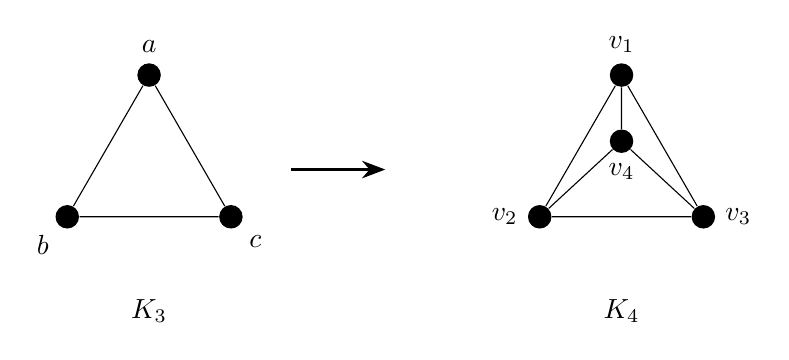
\begin{tikzpicture}[vertex/.style={circle,fill=black,inner sep=3pt}, scale=1.2]
    % Triangle
    \node[vertex, label=above:$a$] (a) at (0,1) {};
    \node[vertex, label=below left:$b$] (b) at (-0.866,-0.5) {};
    \node[vertex, label=below right:$c$] (c) at (0.866,-0.5) {};
    \draw (a) -- (b) -- (c) -- (a);
    \node at (0,-1.5) {$K_3$};
    
    % Arrow
    \draw[-Stealth, very thick] (1.5,0) -- (2.5,0);
    
    % K4
    \begin{scope}[xshift=5cm]
        \node[vertex, label=above:$v_1$] (v1) at (0,1) {};
        \node[vertex, label=left:$v_2$] (v2) at (-0.866,-0.5) {};
        \node[vertex, label=right:$v_3$] (v3) at (0.866,-0.5) {};
        \node[vertex, label=below:$v_4$] (v4) at (0,0.3) {};
        \draw (v1) -- (v2) -- (v3) -- (v1);
        \draw (v1) -- (v4) -- (v2);
        \draw (v3) -- (v4);
        \node at (0,-1.5) {$K_4$};
    \end{scope}
\end{tikzpicture}
\caption{$K_3$ is a minor of $K_4$ (contract any edge)}
\label{fig:simple-minor}
\end{figure}

\subsection{Example of Minors}

To build intuition for minors, we consider one of the most classical examples:
the \textbf{Petersen graph $P_{10}$}. This graph contains both $K_5$ and $K_{3,3}$ as
minors, demonstrating how much structure can be compressed from a larger
graph. Figure~\ref{fig:petersen-minor} illustrates the constructions.

% --- Figure ---
\begin{figure}[htbp]
\centering
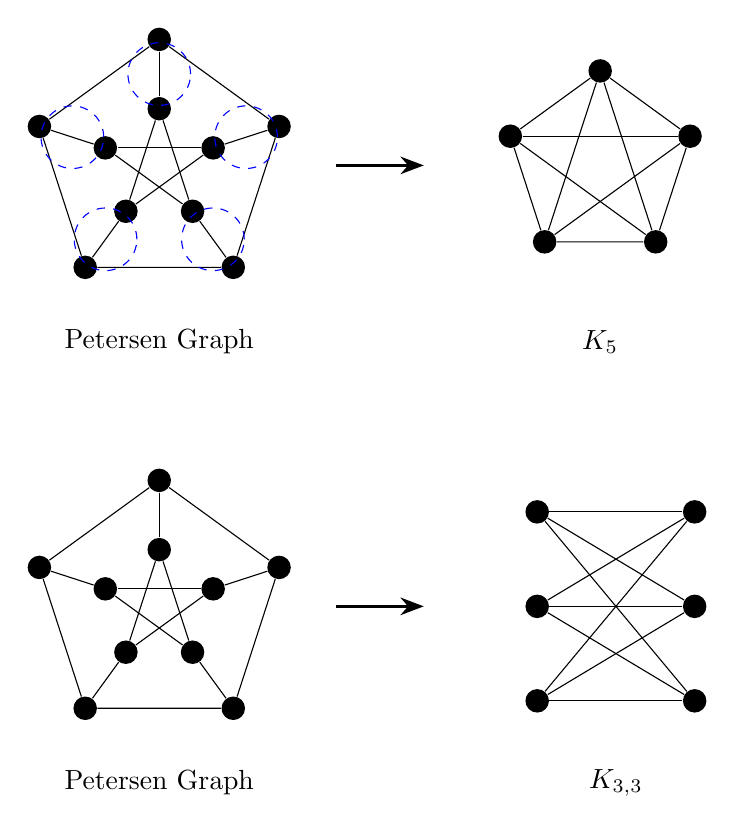
\begin{tikzpicture}[
    vertex/.style={circle,fill=black,inner sep=3pt},
    contract/.style={circle,draw=blue,dashed,inner sep=8pt},
    scale=0.8
]

% Top row - Petersen to K5
\begin{scope}
    % Petersen graph with contraction groups
    % Outer pentagon
    \foreach \i in {0,1,2,3,4} {
        \node[vertex] (outer\i) at ({90+\i*72}:2) {};
    }
    % Inner pentagram
    \foreach \i in {0,1,2,3,4} {
        \node[vertex] (inner\i) at ({90+\i*72}:0.9) {};
    }
    % Draw edges
    \foreach \i in {0,1,2,3,4} {
        \pgfmathtruncatemacro{\next}{mod(\i+1,5)}
        \draw (outer\i) -- (outer\next);
        \pgfmathtruncatemacro{\nexttwo}{mod(\i+2,5)}
        \draw (inner\i) -- (inner\nexttwo);
        \draw (outer\i) -- (inner\i);
    }
    % Contraction circles
    \foreach \i in {0,1,2,3,4} {
        \node[contract] at ({90+\i*72}:1.45) {};
    }
    \node at (0,-2.8) {Petersen Graph};
\end{scope}

% Arrow
\draw[-Stealth, very thick] (2.8,0) -- (4.2,0);

% K5
\begin{scope}[xshift=7cm]
    \foreach \i in {0,1,2,3,4} {
        \node[vertex] (k5\i) at ({90+\i*72}:1.5) {};
    }
    \foreach \i in {0,1,2,3,4} {
        \foreach \j in {0,1,2,3,4} {
            \ifnum\i<\j
                \draw (k5\i) -- (k5\j);
            \fi
        }
    }
    \node at (0,-2.8) {$K_5$};
\end{scope}

% Bottom row - Petersen to K_{3,3}
\begin{scope}[yshift=-7cm]
    % Petersen graph (no contraction circles this time)
    % Outer pentagon
    \foreach \i in {0,1,2,3,4} {
        \node[vertex] (outer2\i) at ({90+\i*72}:2) {};
    }
    % Inner pentagram
    \foreach \i in {0,1,2,3,4} {
        \node[vertex] (inner2\i) at ({90+\i*72}:0.9) {};
    }
    % Draw edges
    \foreach \i in {0,1,2,3,4} {
        \pgfmathtruncatemacro{\next}{mod(\i+1,5)}
        \draw (outer2\i) -- (outer2\next);
        \pgfmathtruncatemacro{\nexttwo}{mod(\i+2,5)}
        \draw (inner2\i) -- (inner2\nexttwo);
        \draw (outer2\i) -- (inner2\i);
    }
    \node at (0,-2.8) {Petersen Graph};
\end{scope}

% Arrow
\draw[-Stealth, very thick] (2.8,-7) -- (4.2,-7);

% K_{3,3}
\begin{scope}[xshift=6cm,yshift=-7cm]
    % Left partition
    \node[vertex] (a1) at (0,1.5) {};
    \node[vertex] (a2) at (0,0) {};
    \node[vertex] (a3) at (0,-1.5) {};
    % Right partition
    \node[vertex] (b1) at (2.5,1.5) {};
    \node[vertex] (b2) at (2.5,0) {};
    \node[vertex] (b3) at (2.5,-1.5) {};
    % Draw all edges
    \foreach \i in {1,2,3} {
        \foreach \j in {1,2,3} {
            \draw (a\i) -- (b\j);
        }
    }
    \node at (1.25,-2.8) {$K_{3,3}$};
\end{scope}

\end{tikzpicture}
\caption{$K_5$ and $K_{3,3}$ are both minors of the Petersen graph}
\label{fig:petersen-minor}
\end{figure}

\subsection{Obtaining $K_5$ as a minor}
Partition the vertices of the Petersen graph into five disjoint pairs, each
forming an edge of a perfect matching. Contracting these five edges yields a
five-vertex graph. The remaining edges between the matched pairs ensure that the
resulting graph is $K_5$.

\subsection{Obtaining $K_{3,3}$ as a minor}
Deleting any one vertex from the outer cycle leaves a $9$-vertex graph from which
a $K_{3,3}$ minor can be obtained by contracting three edges that collapse the
remaining structure into two sets of three vertices.

These examples demonstrate how contraction can highlight deep structural
properties that are not apparent by considering subgraphs alone. This leads us to the idea of minor-closed families.

\begin{definition}[Minor-Closed Family]
A family $\mathcal{F}$ of graphs is \textbf{minor-closed} if whenever $G \in \mathcal{F}$ 
and $H$ is a minor of $G$, then $H \in \mathcal{F}$.
\end{definition}

The set of planar graphs is the canonical example. Deleting edges or contracting edges of a planar graph can never create a non-planar graph. Other examples of \textbf{minor-closed families} include:
\begin{itemize}
    \item \textbf{Forests:} For instance, the star $K_{1,4}$ is a forest. Any minor of this graph remains acyclic, illustrating why the family of forests is minor-closed.
    \item \textbf{Outerplanar Graphs:} A standard example is a triangulated hexagon (a maximal outerplanar graph) where all vertices lie on the boundary of the outer face. This class is characterized by having no $K_4$ or $K_{2,3}$ minors.
\end{itemize}

% --- Figure ---
\begin{figure}[h]
\centering
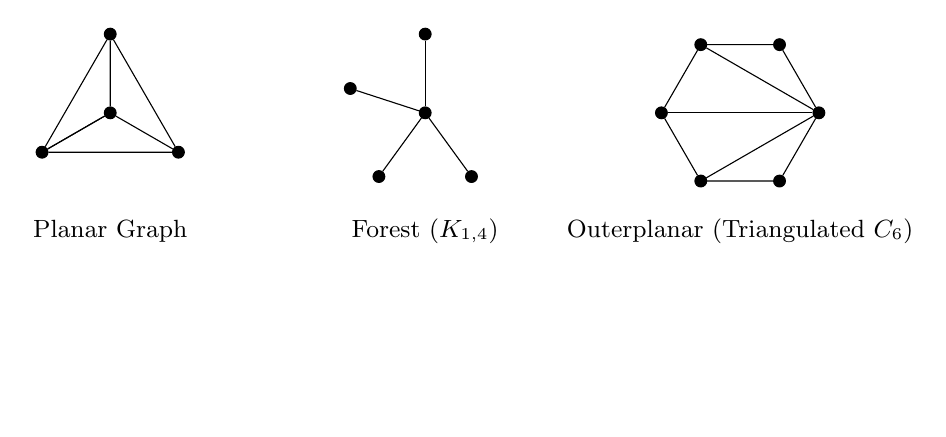
\begin{tikzpicture}[
    scale=1.0,
    every node/.style={circle,fill=black,draw,inner sep=1.5pt},
    baseline=(current bounding box.north)
]

% =============================
% 0. Planar Graph (simple triangulation)
% =============================
\begin{scope}[shift={(0,0)}]
\node (p1) at (90:1) {};
\node (p2) at (210:1) {};
\node (p3) at (330:1) {};

\node (p4) at (0,0) {};

\draw (p1)--(p2)--(p3)--(p1); % outer triangle
\draw (p1)--(p4)--(p2);
\draw (p2)--(p4)--(p3);

\node[draw=none,fill=none,yshift=-1.5cm] {\small Planar Graph};
\end{scope}

% =============================
% 1. Forest (Star K_{1,4})
% =============================
\begin{scope}[shift={(4,0)}]
\node (c) at (0,0) {};
\node (a1) at (90:1) {};
\node (a2) at (162:1) {};
\node (a3) at (234:1) {};
\node (a4) at (306:1) {};
\draw (c) -- (a1);
\draw (c) -- (a2);
\draw (c) -- (a3);
\draw (c) -- (a4);
\node[draw=none,fill=none,yshift=-1.5cm] {\small Forest ($K_{1,4}$)};
\end{scope}

% =============================
% 2. Outerplanar (Triangulated 6-cycle)
% =============================
\begin{scope}[shift={(8,0)}]
\node (b1) at (0:1) {};
\node (b2) at (60:1) {};
\node (b3) at (120:1) {};
\node (b4) at (180:1) {};
\node (b5) at (240:1) {};
\node (b6) at (300:1) {};

\draw (b1)--(b2)--(b3)--(b4)--(b5)--(b6)--(b1);

\draw (b1) -- (b3);
\draw (b1) -- (b4);
\draw (b1) -- (b5);

\node[draw=none,fill=none,yshift=-1.5cm] {\small Outerplanar (Triangulated $C_6$)};
\end{scope}
\end{tikzpicture}
\vspace{-5em} % tightly pulls caption up
\caption{Examples of Minor-Closed Families}
\end{figure}
\vspace{-0.5em}

\subsection{Forbidden Minors}

The concept of minor-closed families naturally leads to the idea of \textbf{forbidden minors}.

\begin{definition}[Forbidden Minors]
For a minor-closed family $\mathcal{F}$, the set of \textbf{forbidden minors} (or \textbf{obstruction set}) is the set of graphs $H$ such that $H \notin \mathcal{F}$, but every proper minor of $H$ is in $\mathcal{F}$.
\end{definition}

By this definition, a graph $G$ belongs to the family $\mathcal{F}$ if and only if $G$ does not contain any forbidden minors as a minor. For forests, the obstruction set is $\{K_3\}$. Any graph without a $K_3$ minor is a forest.

\begin{table}[h]
\centering
\begin{tabular}{l l}
    \toprule
    \textbf{Family} & \textbf{Forbidden Minors} \\
    \midrule
    Forests        & $C_3$ (a single cycle) \\
    Outerplanar    & $K_4, K_{2,3}$\\
    Planar         & $K_5, K_{3,3}$\\
    Linklessly Embeddable & 7 Graphs \\
    \bottomrule
\end{tabular}
\caption{Graph families and their forbidden minors}
\end{table}
\vspace{-1.5em}
% --- History ---
\section{Historical Context and Origins}
\label{sec:history}

The study of graph minors grew out of early 20th-century work on graph embeddings, specifically the problem of characterizing planar graphs. The first major result in this area was not about minors, but about \textbf{topological subdivisions}.

\begin{definition}[Topological Minor]
A graph $H$ is a \textbf{topological minor} of $G$ if a subgraph of $G$ is isomorphic to a \textbf{subdivision} of $H$. A subdivision of $H$ is formed by replacing some edges of $H$ with paths.
\end{definition}

In 1930, \textbf{Kazimierz Kuratowski} published his celebrated theorem characterizing planarity based on this concept.

\begin{theorem}[\textcolor{red}{3}, {Kuratowski}]
A graph $G$ is planar if and only if it does not contain a subgraph that is a subdivision of $K_5$ or $K_{3,3}$.
\end{theorem}

This theorem was a landmark achievement, but the concept of subdivisions is complex to work with. A subdivision of $K_5$ can look very different from $K_5$ itself. In 1937, \textbf{Klaus Wagner} introduced the edge contraction operation and provided a different, simpler characterization of planarity \redcite{9}. This is the result that truly founded graph minor theory.

\begin{theorem}[\textcolor{red}{9}, {Wagner}]
\label{thm:wagner}
A graph $G$ is planar if and only if it does not contain $K_5$ or $K_{3,3}$ as a minor.
\end{theorem}

% --- Figure ---
\begin{figure}[H]
\centering
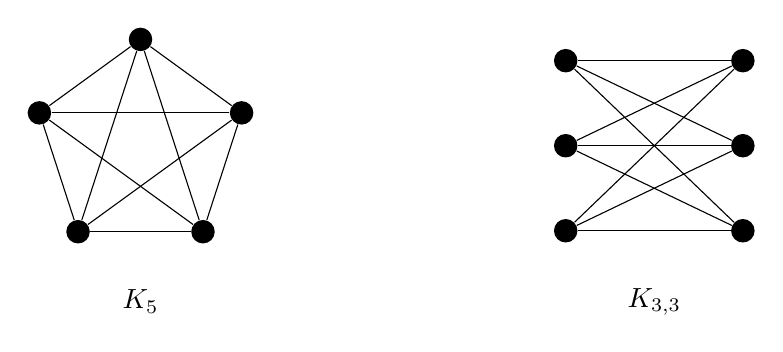
\begin{tikzpicture}[vertex/.style={circle,fill=black,inner sep=3pt}, scale=0.9]
    % K5
    \foreach \i in {0,1,2,3,4} {
        \node[vertex] (k5\i) at ({90+\i*72}:1.5) {};
    }
    \foreach \i in {0,1,2,3,4} {
        \foreach \j in {0,1,2,3,4} {
            \ifnum\i<\j
                \draw (k5\i) -- (k5\j);
            \fi
        }
    }
    \node at (0,-2.2) {$K_5$};
    
    % K_{3,3}
    \begin{scope}[xshift=6cm]
        \node[vertex] (a1) at (0,1.2) {};
        \node[vertex] (a2) at (0,0) {};
        \node[vertex] (a3) at (0,-1.2) {};
        \node[vertex] (b1) at (2.5,1.2) {};
        \node[vertex] (b2) at (2.5,0) {};
        \node[vertex] (b3) at (2.5,-1.2) {};
        \foreach \i in {1,2,3} {
            \foreach \j in {1,2,3} {
                \draw (a\i) -- (b\j);
            }
        }
        \node at (1.25,-2.2) {$K_{3,3}$};
    \end{scope}
\end{tikzpicture}
\caption{The two forbidden minors for planar graphs}
\label{fig:forbidden-planar}
\end{figure}

The minor relationship is more general than the subdivision relationship. If $G$ contains a subdivision of $H$, then $G$ also contains $H$ as a minor (one can contract the internal vertices of the paths). The converse is not true in general. However, for $K_5$ and $K_{3,3}$, the two conditions are equivalent: a graph has a $K_5$ or $K_{3,3}$ minor if and only if it has a $K_5$ or $K_{3,3}$ subdivision \redcite{1}. Wagner's formulation, however, proved to be far more extensible and led to a new wave of inquiry.

The deep connection between graph structure and the minor relation was further highlighted by the \textbf{Hadwiger Conjecture} in 1943 \redcite{2}.

\begin{conjecture}[Hadwiger's Conjecture, 1943 (\textcolor{red}{2}, {Hadwiger})]
\label{conj:hadwiger}
For every integer $k \ge 1$, if a graph $G$ has no $K_k$ minor, then $G$ is $(k-1)$-colorable.
\end{conjecture}

\noindent This conjecture, if true, would be a significant generalization of the Four Color Theorem.
\begin{itemize}
    \item For $k=4$, it states that if $G$ has no $K_4$ minor, it is 3-colorable. This is known to be true.
    \item For $k=5$, it states that if $G$ has no $K_5$ minor, it is 4-colorable. In 1937, Wagner proved that this statement is equivalent to the Four Color Theorem \redcite{9}. Since the Four Color Theorem was proven in 1976 (with subsequent formal verification), the $k=5$ case of Hadwiger's Conjecture is also true.
    \item For $k=6$, the conjecture states that a graph with no $K_6$ minor is 5-colorable. This was proven by Robertson, Seymour, and Thomas in 1993 \redcite{8}, using techniques related to the Four Color Theorem.
\end{itemize}
For $k \ge 7$, the conjecture remains one of the most significant open problems in graph theory. The persistence and difficulty of this conjecture demonstrated that the minor relation was tied to fundamental properties of graphs, motivating decades of research that culminated in the work of Robertson and Seymour.

% --- Key Results (Wagner) ---
\section{Wagner's Theorem}
\label{sec:wagner}

Wagner's Theorem (Theorem \ref{thm:wagner}) is the cornerstone of graph minor theory. It provides a simple and elegant characterization for the infinite family of planar graphs. The power of the theorem lies in its `` if and only if '' nature. It is clear that $K_5$ and $K_{3,3}$ are not planar, and since planarity is a minor-closed property, any graph containing them as a minor also cannot be planar. The difficult part is proving the other direction: that every non-planar graph must contain one of these two graphs as a minor.

\subsection{Proof Sketch of Wagner's Theorem}

A full proof of Wagner's theorem is highly non-trivial and relies on deep structural results. One common approach involves Kuratowski's other theorem about 3-connected graphs, but a more direct proof route, developed by Wagner himself \redcite{9}, relies on the concept of graph connectivity and minimal counterexamples. We provide a brief sketch of the ideas involved.

The proof proceeds by induction on the number of vertices. We assume the theorem holds for all graphs with fewer vertices than $G$. We can also assume $G$ is a minimal non-planar graph, meaning $G$ is not planar, but every proper minor of $G$ is planar. If $G$ is such a graph, it must not have $K_5$ or $K_{3,3}$ as a minor (otherwise, a proper minor of $G$ would be $K_5$ or $K_{3,3}$, which are non-planar, contradicting minimality). The goal is to show that the only such graphs are $K_5$ and $K_{3,3}$ themselves.

\begin{enumerate}
    \item \textbf{Connectivity:} A minimal non-planar graph $G$ must be 3-connected. If $G$ had a 1- or 2-vertex cut, we could decompose $G$ into smaller graphs $G_1, G_2$. If $G$ is non-planar, at least one of $G_1$ or $G_2$ must be non-planar. This non-planar component would be a proper minor of $G$, and by induction, would contain a $K_5$ or $K_{3,3}$ minor, which would also be a minor of $G$.

    \item \textbf{Wagner's Lemma:} The core of the proof is a structural lemma by Wagner. It states that any 3-connected graph $G$ that does not contain a $K_5$ minor can be constructed in a specific way. Such graphs can be formed by repeatedly pasting simpler graphs together along triangles, an operation known as a 3-sum. A 3-sum of two graphs $G_1$ and $G_2$ is obtained by identifying a triangle in $G_1$ with a triangle in $G_2$, possibly deleting some of the resulting parallel edges. For instance, if $G_1$ contains triangle $\{a, b, c\}$ and $G_2$ contains triangle $\{x, y, z\}$, the 3-sum merges these by identifying $a$ with $x$, $b$ with $y$, and $c$ with $z$, creating a single shared triangular structure. This operation glues the graphs together along a 3-cycle while preserving 3-connectivity.

    \item \textbf{The Final Step:} The proof then shows that any 3-connected graph $G$ built this way, which also does not have a $K_{3,3}$ minor, must be planar.
\end{enumerate}

Therefore, if $G$ is a 3-connected graph that is non-planar, it must contain either a $K_5$ minor or a $K_{3,3}$ minor. This sketch glosses over significant technical detail, but it illustrates the strategy: using connectivity to constrain the structure of a minimal counterexample.

The significance of Wagner's Theorem is not just its result, but its method. It provided a finite basis for the property of planarity. It begged the question: what other graph properties have a finite forbidden minor characterization?
\begin{itemize}
    \item The family of outerplanar graphs is characterized by forbidding $K_4$ and $K_{2,3}$.
    \item The family of graphs that are \textbf{apex} (planar after deleting one vertex) is also known to have a finite, though very large, set of forbidden minors.
\end{itemize}
For decades, it was an open question whether every minor-closed family of graphs had a finite forbidden minor characterization.

% --- Graph Minor Theorem ---
\section{The Graph Minor Theorem}
\label{sec:gmt}

This question was answered definitively by \textbf{Neil Robertson and Paul Seymour} in a series of 20 papers spanning over two decades (1983-2004), collectively known as the \textbf{Graph Minors} series. Their main result, the Robertson-Seymour Theorem (or Graph Minor Theorem), is one of the deepest and most profound results in all of combinatorics.

The theorem is not usually stated in terms of forbidden minors, but rather as a statement about the ordering of graphs.

\begin{definition}[Well-Quasi-Ordering]
A partial order $\preceq$ on a set $S$ is a \textbf{well-quasi-ordering (WQO)} if, for any infinite sequence of elements $s_1, s_2, s_3, \ldots$ from $S$, there exist indices $i < j$ such that $s_i \preceq s_j$.
\end{definition}

A WQO does not contain any \textbf{infinite antichains} (an infinite set of pairwise incomparable elements). For intuition, a simple example of a well-quasi-ordering is the natural numbers 
under the usual order $\le$: any infinite sequence of natural numbers must contain 
an increasing pair, so no infinite antichain exists.

The Robertson-Seymour Theorem states that the minor relation is a WQO on the set of all finite graphs.

\begin{theorem}[Graph Minor Theorem, 2004 (\textcolor{red}{6}, {Robertson and Seymour})]
\label{thm:gmt}
The set of all finite graphs is well-quasi-ordered by the graph minor relation $\preceq$.
\end{theorem}

This theorem is \textbf{non-constructive} in the sense that its proof does not provide a general method for finding the pair $i, j$. It merely proves that such a pair must exist. The proof is incredibly complex, running over 500 pages, and relies on developing a massive new structural theory for graphs.

\subsection{The Forbidden Minor Characterization}

The power of this WQO result becomes apparent when we consider what it means for minor-closed families: if no infinite sequence of graphs can be pairwise incomparable under the minor relation, then the set of minimal obstructions for any minor-closed property must be finite. This leads directly to the following corollary.

\begin{corollary}
\label{cor:forbidden}
Every minor-closed family of graphs $\mathcal{F}$ can be characterized by a finite set of forbidden minors $\mathcal{O}$.
\end{corollary}

\noindent \textit{Proof Sketch of Corollary \ref{cor:forbidden} from Theorem \ref{thm:gmt}}

Let $\mathcal{F}$ be a minor-closed family of graphs. Let $\mathcal{O}$ be the set of all minimal graphs that are not in $\mathcal{F}$. That is, $H \in \mathcal{O}$ if $H \notin \mathcal{F}$, but every proper minor of $H$ is in $\mathcal{F}$. By definition, $\mathcal{F}$ is exactly the set of graphs that do not contain any graph from $\mathcal{O}$ as a minor. We need to show that $\mathcal{O}$ is finite.

Suppose, for the sake of contradiction, that $\mathcal{O}$ is infinite. Let $\mathcal{O} = \{H_1, H_2, H_3, \ldots\}$ be an infinite sequence of distinct graphs from $\mathcal{O}$.

By the Robertson-Seymour Theorem (Theorem \ref{thm:gmt}), the set of finite graphs is well-quasi-ordered by the minor relation. Therefore, there must exist indices $i < j$ such that $H_i \preceq H_j$. 

But $H_j$ is in the obstruction set $\mathcal{O}$, which means it is a minimal graph not in $\mathcal{F}$. And $H_i$ is a proper minor of $H_j$ (it must be proper, as the $H_k$ are distinct).
Since $H_j$ is minimal, every proper minor of $H_j$ must be in $\mathcal{F}$. This means $H_i$ must be in $\mathcal{F}$. However, $H_i$ is also in the set $\mathcal{O}$, which means $H_i \notin \mathcal{F}$. This is a contradiction.

Therefore, our initial assumption that $\mathcal{O}$ is infinite must be false. The obstruction set $\mathcal{O}$ must be finite.

The significance of this result is hard to overstate. It is a meta-theorem that proves the existence of a finite characterization for countless graph properties, even ones no one has studied yet. For any property $P$ that is hereditary under minors (e.g., being embeddable on a torus, being a linkless embedding in 3D space, etc.), Robertson and Seymour's Corollary \redcite{6} guarantees that there is a finite list of forbidden graphs that defines $P$.

\subsection{Graph Structure and Tree-Width}

The proof of the Graph Minor Theorem is not just a single argument, but the development of an entire structural graph theory. A central concept created for the proof is \textbf{tree-width}.

\begin{definition}[Tree--Width]
    The tree-width of a graph $G$ is the smallest width of any tree decomposition of $G$. A \textbf{tree decomposition} of $G$ is a tree $T$ where each node contains a subset of $V(G)$ (called a bag), such that:
\end{definition}

\begin{enumerate}
    \item Every vertex of $G$ appears in at least one bag
    \item For every edge $\{u,v\}$ in $G$, some bag contains both $u$ and $v$
    \item For each vertex $v \in V(G)$, the bags containing $v$ form a connected subtree of $T$
\end{enumerate}
The width of a decomposition is the size of its largest bag minus one. Intuitively, tree-width measures how \textbf{tree-like} a graph is.

% --- Figure ---
\begin{figure}[H]
\centering
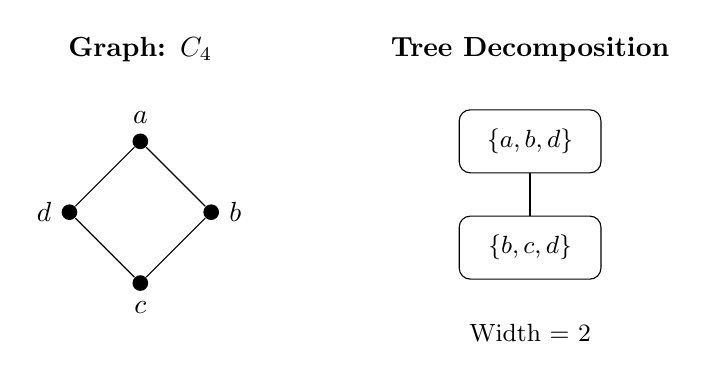
\begin{tikzpicture}[
    vertex/.style={circle,fill=black,inner sep=2pt},
    bag/.style={rectangle,draw,rounded corners,minimum width=1.8cm,minimum height=0.8cm},
    scale=0.9
]
    % Original graph - a simple cycle C4
    \begin{scope}
        \node at (0,2.8) {\textbf{Graph: $C_4$}};
        \node[vertex,label=above:$a$] (a) at (0,1.5) {};
        \node[vertex,label=right:$b$] (b) at (1,0.5) {};
        \node[vertex,label=below:$c$] (c) at (0,-0.5) {};
        \node[vertex,label=left:$d$] (d) at (-1,0.5) {};
        \draw (a) -- (b) -- (c) -- (d) -- (a);
    \end{scope}
    
    % Tree decomposition - corrected
    \begin{scope}[xshift=5.5cm]
        \node at (0,2.8) {\textbf{Tree Decomposition}};
        \node[bag] (t1) at (0,1.5) {\small $\{a,b,d\}$};
        \node[bag] (t2) at (0,0) {\small $\{b,c,d\}$};
        \draw[thick] (t1) -- (t2);
        \node at (0,-1.2) {\small Width = 2};
    \end{scope}
\end{tikzpicture}
\caption{A cycle $C_4$ and its tree decomposition of width 2}
\label{fig:tree-decomposition}
\end{figure}

\textbf{Examples:}
\begin{itemize}
    \item A tree has tree-width 1 (each bag contains an edge)
    \item A cycle $C_n$ has tree-width 2
    \item A $k \times k$ grid has tree-width $k$
    \item A complete graph $K_n$ has tree-width $n-1$
\end{itemize}

A major part of the Robertson-Seymour proof, often called the \textbf{Grid Minor Theorem}, shows that any graph with sufficiently large tree-width must contain a large grid graph as a minor \redcite{7}. Specifically, for any $k$, there exists a function $f(k)$ such that every graph with tree-width at least $f(k)$ contains the $k \times k$ grid as a minor.

A second key part involves showing that any graph $G$ that does not have a specific minor $H$ (i.e., is $H$-minor-free) must have a specific structure. The \textbf{structure theorem} states that any such graph $G$ can be decomposed into a tree-structure of graphs that are almost-embedded on a simpler surface (a surface on which $H$ cannot be embedded) \redcite{6}. This provides a structural characterization: $H$-minor-free graphs have bounded complexity relative to the surface structure of $H$.

\section{Applications}
\label{sec:applications}

The Graph Minor Theorem is not just a theoretical curiosity; it has profound implications for our understanding of graph properties and their decidability, even though the proof itself is non-constructive.

\subsection{Algorithmic Implications}

A major consequence of the Graph Minor Theorem is that it establishes the decidability of membership for all minor-closed graph families.

Robertson and Seymour proved that for any fixed graph $H$, testing whether a given graph $G$ has $H$ as a minor ($H \preceq G$) can be done in polynomial time. Specifically, the time complexity is $O(n^3)$ for a graph $G$ with $n$ vertices.
This result, combined with Corollary \ref{cor:forbidden}, yields a striking meta-theorem:

\begin{theorem}[\textcolor{red}{7}, Robertson and Seymour]
\label{thm:membership}
For any minor-closed family of graphs $\mathcal{F}$, there is a polynomial-time algorithm to test if a graph $G$ belongs to $\mathcal{F}$.
\end{theorem}

This is a powerful and far-reaching result. It guarantees that questions like ``Is this graph planar?'', ``Is this graph embeddable on a torus?'', and infinitely many other structural properties are decidable in polynomial time.

However, there is an important caveat: the theorem is non-constructive. While the Graph Minor Theorem guarantees that the obstruction set $\mathcal{O}$ is finite, it does not provide a method to find $\mathcal{O}$ explicitly. Even for relatively simple families, the obstruction set can be enormous. For instance, while linklessly embeddable graphs are characterized by exactly 7 minimal forbidden minors \redcite{5}, the obstruction set for graphs embeddable on a torus is known to contain more than 17,000 forbidden minors \redcite{4}. This demonstrates the dramatic gap between theoretical decidability and practical computability.

Despite this limitation, the theorem represents a fundamental contribution to structural graph theory, establishing that the elegant characterization of minor-closed families by forbidden minors translates directly into algorithmic tractability.

% --- Conclusion ---
\section*{Conclusion}
\label{sec:conclusion}

The theory of graph minors offers a profound and unifying perspective on the structure of graphs. It elevates the simple, intuitive operations of deletion and contraction into a powerful ordering relation. This framework, first hinted at by Wagner's elegant characterization of planar graphs \redcite{9}, transforms the complex topological problem of planarity into a simple check for two forbidden structures, $K_5$ and $K_{3,3}$.

The full potential of this perspective was realized in the monumental Graph Minor Theorem by Robertson and Seymour \redcite{6}. By proving that the set of finite graphs is well-quasi-ordered under the minor relation, they showed that every minor-closed property from planarity to embeddability on any fixed surface is characterized by a finite list of forbidden minors.

This result fundamentally changed the landscape of structural graph theory. It guarantees the existence of finite characterizations for an endless number of graph families, while the deep structural theory developed for its proof (such as the concept of tree-width) has become a field of study in its own right. Furthermore, its algorithmic consequences, while non-constructive, provide a sweeping guarantee of polynomial-time decidability for all minor-closed properties.

From Wagner's initial insight to the comprehensive theory of Robertson and Seymour, the study of graph minors has demonstrated that by asking simple questions about how graphs relate to each other, we can uncover the deepest and most fundamental principles of their structure.

% --- Bibliography ---
\begin{thebibliography}{99}

\bibitem{1} Diestel, R. \textit{Graph Theory}. 5th ed. Springer, 2017.

\bibitem{2} Hadwiger, H. Über eine Klassifikation der Streckenkomplexe. \textit{Vierteljahresschrift der Naturforschenden Gesellschaft in Zürich}, 88:133-142, 1943.

\bibitem{3} Kuratowski, K. Sur le problème des courbes gauches en topologie. \textit{Fundamenta Mathematicae}, 15:271-283, 1930.

\bibitem{4} Myrvold, W. and J. Woodcock. A large set of torus obstructions and how they were discovered. \textit{Electronic Journal of Combinatorics}, 25(1):P1.16, 2018.

\bibitem{5} Robertson, N., P. D. Seymour, and R. Thomas. Linkless embeddings of graphs in 3-space. \textit{Bulletin of the American Mathematical Society}, 28(1):84-89, 1993.

\bibitem{6} Robertson, N. and P. D. Seymour. Graph minors. XX. Wagner's conjecture. \textit{Journal of Combinatorial Theory, Series B}, 92(2):325-357, 2004.

\bibitem{7} Robertson, N. and P. D. Seymour. Graph minors. XIII. The disjoint paths problem. \textit{Journal of Combinatorial Theory, Series B}, 63(1):65-110, 1995.

\bibitem{8} Robertson, N., P. D. Seymour, and R. Thomas. Hadwiger's conjecture for $K_6$-free graphs. \textit{Combinatorica}, 13(3):279-361, 1993.

\bibitem{9} Wagner, K. Über eine Eigenschaft der ebenen Komplexe. \textit{Mathematische Annalen}, 114:570-590, 1937.

\end{thebibliography}

\end{document}